\documentclass[border=4pt]{standalone}
\usepackage[T1]{fontenc}
\usepackage{stix}
\usepackage{amsmath,amssymb,graphicx,tikz}
\usetikzlibrary{positioning,arrows.meta,shapes.geometric,fit}
\begin{document}
\resizebox{173.8mm}{!}{%
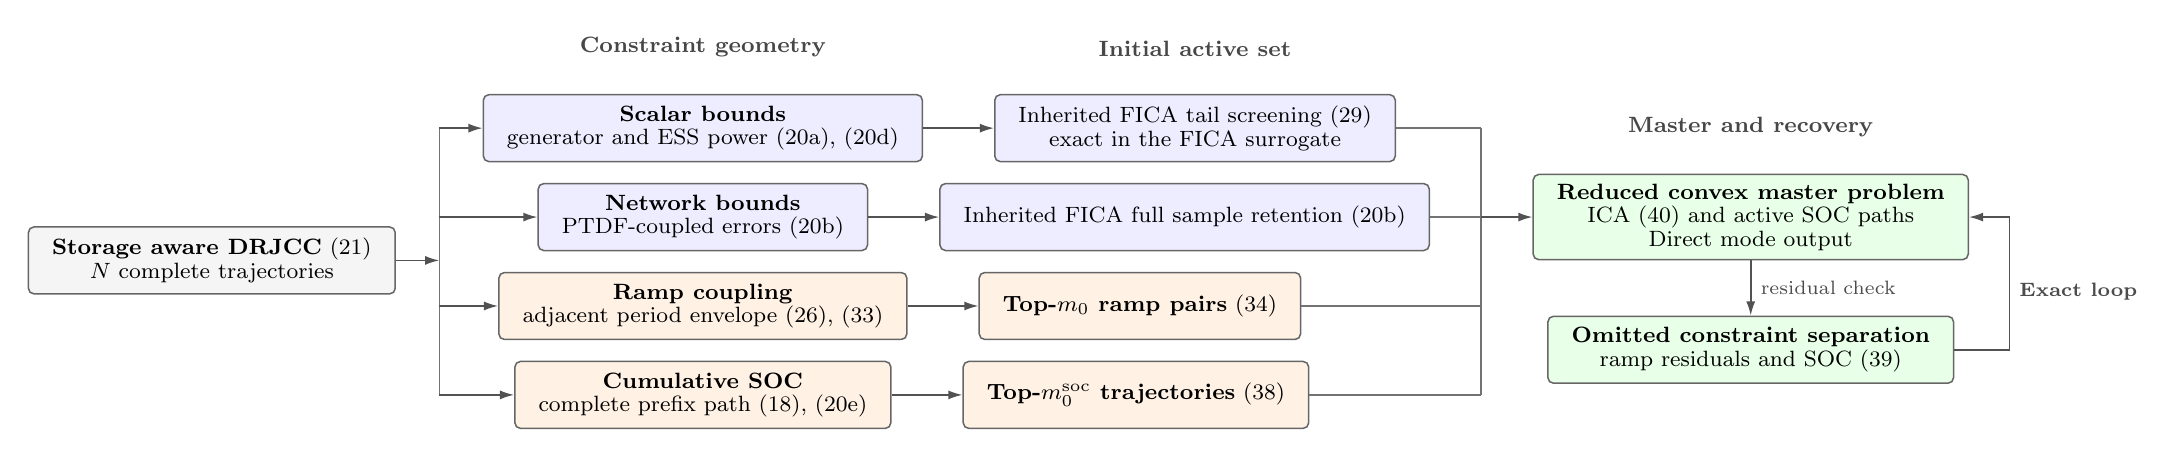
\begin{tikzpicture}[
font=\footnotesize,
node distance=2.6mm and 8mm,
box/.style={rectangle, rounded corners=2pt, draw=black!60, line width=0.55pt,
minimum height=8.5mm, align=center, inner xsep=3mm},
source/.style={box, fill=black!4, minimum width=29mm},
instant/.style={box, fill=blue!7, minimum width=34mm},
temporal/.style={box, fill=orange!10, minimum width=34mm},
solve/.style={box, fill=green!9, minimum width=39mm},
flow/.style={-{Latex[length=1.8mm,width=1.15mm]}, draw=black!68, line width=0.6pt},
bus/.style={draw=black!55, line width=0.55pt},
stage/.style={font=\footnotesize\bfseries, text=black!72, align=center}]

\node[source] (model) {\textbf{Storage aware DRJCC}~(21)\\[-1pt]\footnotesize $N$ complete trajectories};

\node[instant, right=11mm of model, yshift=16.8mm] (scalar)
  {\textbf{Scalar bounds}\\[-1pt]\footnotesize generator and ESS power~(20a), (20d)};
\node[instant, below=of scalar] (network)
  {\textbf{Network bounds}\\[-1pt]\footnotesize PTDF-coupled errors~(20b)};
\node[temporal, below=of network] (ramp)
  {\textbf{Ramp coupling}\\[-1pt]\footnotesize adjacent period envelope~(26), (33)};
\node[temporal, below=of ramp] (soc)
  {\textbf{Cumulative SOC}\\[-1pt]\footnotesize complete prefix path~(18), (20e)};

\node[instant, right=9mm of scalar] (tails)
  {Inherited FICA tail screening~(29)\\[-1pt]\footnotesize exact in the FICA surrogate};
\node[instant, right=9mm of network] (full)
  {Inherited FICA full sample retention~(20b)};
\node[temporal, right=9mm of ramp] (rinit)
  {\textbf{Top-$m_0$ ramp pairs}~(34)};
\node[temporal, right=9mm of soc] (sinit)
  {\textbf{Top-$m_0^{\mathrm{soc}}$ trajectories}~(38)};

\node[solve, right=13mm of full] (master)
  {\textbf{Reduced convex master problem}\\[-1pt]\footnotesize ICA~(40) and active SOC paths\\[-1pt]\footnotesize Direct mode output};
\node[solve, below=7mm of master] (check)
  {\textbf{Omitted constraint separation}\\[-1pt]\footnotesize ramp residuals and SOC~(39)};

\node[stage, above=3.5mm of scalar] {Constraint geometry};
\node[stage, above=3.5mm of tails] {Initial active set};
\node[stage, above=3.5mm of master] {Master and recovery};

\coordinate (split) at ([xshift=5.5mm]model.east);
\draw[bus] (split |- scalar.west) -- (split |- soc.west);
\draw[flow] (model.east) -- (split |- model.east);
\draw[flow] (split |- scalar.west) -- (scalar.west);
\draw[flow] (split |- network.west) -- (network.west);
\draw[flow] (split |- ramp.west) -- (ramp.west);
\draw[flow] (split |- soc.west) -- (soc.west);

\draw[flow] (scalar) -- (tails);
\draw[flow] (network) -- (full);
\draw[flow] (ramp) -- (rinit);
\draw[flow] (soc) -- (sinit);

\coordinate (merge) at ([xshift=6.5mm]full.east);
\draw[bus] (merge |- tails.east) -- (merge |- sinit.east);
\draw[bus] (tails.east) -- (merge |- tails.east);
\draw[bus] (full.east) -- (merge |- full.east);
\draw[bus] (rinit.east) -- (merge |- rinit.east);
\draw[bus] (sinit.east) -- (merge |- sinit.east);
\draw[flow] (merge |- master.west) -- (master.west);

\draw[flow] (master) -- node[right, font=\scriptsize, text=black!70]
  {residual check} (check);
\draw[flow] (check.east) -- ++(7mm,0) |- node[pos=0.22, right,
  font=\scriptsize\bfseries, text=black!70] {Exact loop} (master.east);
\end{tikzpicture}
}
\end{document}
